\documentclass[11pt,a4paper]{article}
\usepackage[T1]{fontenc}
\usepackage[utf8]{inputenc}
\usepackage{lmodern}
\usepackage[a4paper,margin=2.4cm]{geometry}
\usepackage{microtype}
\usepackage{setspace}
\usepackage{amsmath}
\usepackage{graphicx}
\usepackage{booktabs,tabularx,multirow,makecell}
\usepackage[table]{xcolor}
\usepackage{caption}
\usepackage{float}
\usepackage{enumitem}
\usepackage{tikz}
\usetikzlibrary{arrows.meta,positioning,decorations.pathreplacing,calc}
\usepackage{titlesec}
\usepackage{fancyhdr}
\usepackage{lastpage}
\usepackage[hidelinks]{hyperref}

\graphicspath{{figs/}}
\setstretch{1.15}
\setlength{\parindent}{0pt}
\setlength{\parskip}{0.55em}
\captionsetup{font=small,labelfont=bf,labelsep=period}
\setlist{itemsep=0.15em,topsep=0.3em}
\titleformat{\section}{\normalfont\large\bfseries}{\thesection}{0.8em}{}
\titleformat{\subsection}{\normalfont\normalsize\bfseries}{\thesubsection}{0.8em}{}
\titlespacing*{\section}{0pt}{1.3em}{0.5em}
\titlespacing*{\subsection}{0pt}{0.9em}{0.3em}

\definecolor{cnx}{HTML}{2A78D6}
\definecolor{rn}{HTML}{EB6834}
\definecolor{ink}{HTML}{1F2328}
\definecolor{boxfill}{HTML}{EEF4FB}

\pagestyle{fancy}
\fancyhf{}
\fancyhead[L]{\small\itshape Dahal --- Lesion-grouped evaluation of dermoscopic lesion classification}
\fancyhead[R]{\small\itshape Preprint, not peer reviewed}
\fancyfoot[C]{\small \thepage\ of \pageref{LastPage}}
\renewcommand{\headrulewidth}{0.4pt}
\newcommand{\pct}{\,\%}

\begin{document}

% ------------------------------------------------------------------ title block
\begin{center}
{\LARGE\bfseries Lesion-grouped evaluation of deep learning for seven-class dermoscopic skin lesion classification, with a validation-tuned melanoma screening threshold\par}
\vspace{1.0em}
{\large Subarna Dahal\par}
\vspace{0.3em}
{\small Correspondence: \href{mailto:dahalsubarna9@gmail.com}{dahalsubarna9@gmail.com}\quad$\cdot$\quad Code and data: \url{https://github.com/subarna007/skin-lesion-classification-isic2018}\par}
\vspace{0.3em}
{\small Version of 18 November 2026\par}
\end{center}
\vspace{0.4em}

\noindent\rule{\textwidth}{0.4pt}

{\small
\textbf{Abstract}

\textbf{Background.} Deep learning models for dermoscopic skin lesion classification are often evaluated on random image-level splits of HAM10000, a dataset that contains several images of the same lesion. Such splits let near-duplicate images fall on both sides and can overstate performance. Melanoma sensitivity, the figure that matters most for triage, is also often reported only at the default decision rule.

\textbf{Methods.} I used the 10,015 images of the ISIC 2018 Task 3 training set (HAM10000) with a split grouped by lesion identifier and stratified by class: 6,987 training, 1,520 validation and 1,508 test images, with no lesion in more than one partition. I compared a ResNet-50 baseline (224\,px, class-weighted cross-entropy, light augmentation) with ConvNeXt-Tiny (384\,px, class-balanced sampling, strong augmentation, flip test-time augmentation). Models were selected on validation balanced accuracy. A melanoma screening threshold was fixed on the validation set for 90\pct{} sensitivity before the test set was used. Test metrics carry 95\pct{} bootstrap confidence intervals (1,000 resamples). Class-specific Grad-CAM maps were inspected, and the model was embedded in a prototype triage application.

\textbf{Results.} ConvNeXt-Tiny reached a balanced accuracy of 76.7\pct{} (95\pct{} CI 72.2--80.9\pct) against 71.3\pct{} (66.4--75.6\pct) for the baseline, and a macro-averaged AUC of 0.966 (0.957--0.974) against 0.932 (0.919--0.944). Melanoma sensitivity as the top prediction rose from 62.2\pct{} to 82.1\pct{} (76.1--87.7\pct). At the validation-tuned threshold, the model flagged 94.2\pct{} (90.4--97.5\pct) of test melanomas at 75.5\pct{} specificity. Actinic keratosis sensitivity fell from 76.1\pct{} to 50.0\pct, and nevi predicted as melanoma were the most frequent error.

\textbf{Conclusions.} Under a leakage-free protocol, a modern convolutional architecture with class-balanced sampling markedly improved melanoma detection over a capstone-style baseline, and a threshold chosen on validation data transferred to the test set. External validation on images from South Asian clinics is needed before any clinical use.

\textbf{Keywords:} skin lesion classification; dermoscopy; melanoma; deep learning; ConvNeXt; data leakage; class imbalance; explainability; HAM10000
}

\noindent\rule{\textwidth}{0.4pt}

% ------------------------------------------------------------------ 1
\section{Introduction}
Melanoma caused an estimated 331,722 new cases and 58,667 deaths worldwide in 2022 \cite{bray2024,iarc2024}. Survival depends strongly on tumour thickness at diagnosis, so early recognition matters. Specialist capacity is uneven: a 2026 survey of 158 countries found a mean of 0.37 dermatologists per 100,000 people in low-income countries, with 91\pct{} of them working in urban areas \cite{freeman2026}. In such settings, most skin lesions are first seen by general practitioners and health assistants.

Deep learning has reached dermatologist-level performance on curated dermoscopic image sets \cite{esteva2017,haenssle2018,tschandl2019}. In the ISIC 2018 reader study, the top algorithms made more correct diagnoses than 27 experienced dermatologists, but their advantage shrank on images from centres not represented in training \cite{tschandl2019}. Such results make decision support for non-specialists plausible, provided the reported performance reflects what a model will do on new patients.

HAM10000, released as the ISIC 2018 Task 3 training set, is the most widely used public benchmark for seven-class dermoscopic classification \cite{codella2019,tschandl2018}. It contains 10,015 images of 7,470 lesions, so many lesions appear more than once. When studies split it at random by image, photographs of the same lesion can land in both training and test sets. Duplicates across ISIC partitions \cite{cassidy2022} and lesion-level leakage in a derived benchmark \cite{abhishek2025} have been documented, and both inflate reported performance. Many studies also report overall accuracy, which on HAM10000 is dominated by the nevus class (67\pct{} of images), rather than balanced accuracy, the official challenge metric \cite{codella2019}.

This work began as an MSc capstone project that trained a ResNet-50 on an image-level split. It reported 76.7\pct{} accuracy but only 36.3\pct{} melanoma recall, and model selection and evaluation used the same split. Here I rebuild the pipeline with a stricter protocol and ask how much of that weakness a modern architecture and better imbalance handling can fix. My contributions are:
\begin{enumerate}
  \item a lesion-grouped, class-stratified train / validation / test split of HAM10000, released with the code so that results can be reproduced and compared;
  \item a controlled comparison of a capstone-style ResNet-50 baseline with ConvNeXt-Tiny trained with class-balanced sampling, both evaluated once on the same held-out test set with bootstrap confidence intervals;
  \item a melanoma screening operating point fixed on validation data before testing, reporting the sensitivity and specificity a triage user would actually experience;
  \item an open-source prototype that combines the classifier with class-specific Grad-CAM, image-based ABCD descriptors and similar-case retrieval, illustrating how the model could support referral decisions in a district hospital.
\end{enumerate}

% ------------------------------------------------------------------ 2
\section{Related work}
\textbf{Deep learning for dermoscopy.} Esteva et al.\ trained an Inception network on 129,450 clinical images and matched 21 dermatologists on two binary tasks \cite{esteva2017}. Haenssle et al.\ showed that a CNN outperformed most of 58 dermatologists in melanoma recognition from dermoscopic images \cite{haenssle2018}. The ISIC 2018 challenge moved the field to seven-class diagnosis on HAM10000, ranked by balanced multiclass accuracy \cite{codella2019}, and its reader study compared 139 algorithms with 511 human readers \cite{tschandl2019}. Residual networks \cite{he2016} were the common backbone of that period; ConvNeXt \cite{liu2022} modernises the convolutional design and is a strong ImageNet-pretrained baseline at moderate cost.

\textbf{Data quality and leakage.} Cassidy et al.\ analysed the ISIC releases from 2016 to 2020, found many duplicate images, including duplicates spread across training and test sets, and proposed a curated deduplicated set \cite{cassidy2022}. Abhishek et al.\ showed that DermaMNIST, a widely used benchmark derived from HAM10000, placed images of the same lesion in different partitions, and released corrected splits \cite{abhishek2025}. Grouping by lesion or patient identifier is the standard remedy in medical imaging, but random image-level splits of HAM10000 remain common in published work and student projects alike.

\textbf{Imbalance and operating points.} HAM10000 is heavily imbalanced: nevi make up 67\pct{} of images and dermatofibroma 1.1\pct. Common remedies are class-weighted losses, resampling and augmentation. Because the default argmax rule rarely matches the sensitivity a screening use needs, a clinically meaningful operating point should be chosen on validation data and then reported on test data, rather than tuned on the test set.

\textbf{Explainability and fairness.} Grad-CAM \cite{selvaraju2017} is widely used to show which image regions drive a CNN's prediction, although a plausible map does not prove clinically valid reasoning. Daneshjou et al.\ found that dermatology AI models lost 27--36\pct{} of their ROC-AUC on a curated set with diverse skin tones and uncommon diseases, performing worst on dark skin \cite{daneshjou2022}. This is directly relevant to deployment in South Asia, since HAM10000 comes mainly from European and Australian clinics \cite{tschandl2018}.

% ------------------------------------------------------------------ 3
\section{Materials and methods}
\subsection{Data}
I used the HAM10000 dataset \cite{tschandl2018}, identical to the ISIC 2018 Task 3 training set \cite{codella2019}: 10,015 dermoscopic images of 7,470 lesions, each labelled with one of seven diagnoses (Supplementary Figure~S1). Labels were confirmed by histopathology in more than half of cases and by follow-up, expert consensus or confocal microscopy otherwise \cite{tschandl2018}. The images and the metadata file mapping each image to its lesion identifier were taken from the public Kaggle mirror of HAM10000. The official ISIC 2018 test labels were not used. 1,956 lesions have more than one image.

\subsection{Lesion-grouped split}
Images were partitioned with scikit-learn's StratifiedGroupKFold \cite{pedregosa2011} into 20 folds (shuffled, seed 42), grouped by lesion identifier and stratified by diagnosis. Three folds formed the test set, three the validation set and the remaining 14 the training set (Figure~\ref{fig:split}). No lesion appears in more than one partition. Table~\ref{tab:split} gives the class counts. The exact assignment of every image is released with the code.

\begin{figure}[ht]
\centering
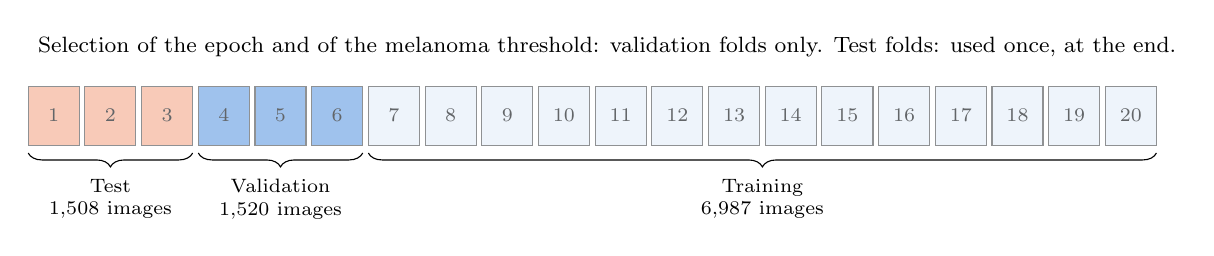
\begin{tikzpicture}[x=0.72cm, y=1cm]
\foreach \i in {1,...,20} {
  \pgfmathsetmacro{\col}{\i<=3 ? "rn!35" : (\i<=6 ? "cnx!45" : "boxfill")}
  \fill[\col] (\i-1,0) rectangle (\i-0.1,0.75);
  \draw[ink!50] (\i-1,0) rectangle (\i-0.1,0.75);
  \node[font=\scriptsize, ink!70] at (\i-0.55,0.375) {\i};
}
\draw[decorate, decoration={brace, amplitude=5pt, mirror}] (0,-0.1) -- (2.9,-0.1) node[midway, below=6pt, font=\scriptsize, align=center] {Test\\1,508 images};
\draw[decorate, decoration={brace, amplitude=5pt, mirror}] (3,-0.1) -- (5.9,-0.1) node[midway, below=6pt, font=\scriptsize, align=center] {Validation\\1,520 images};
\draw[decorate, decoration={brace, amplitude=5pt, mirror}] (6,-0.1) -- (19.9,-0.1) node[midway, below=6pt, font=\scriptsize, align=center] {Training\\6,987 images};
\node[font=\footnotesize, anchor=west, align=left] at (0,1.25) {Selection of the epoch and of the melanoma threshold: validation folds only. Test folds: used once, at the end.};
\end{tikzpicture}
\caption{Study design. The 10,015 images were divided into 20 folds grouped by lesion and stratified by class, so all images of a lesion fall in one fold. Folds 1--3 form the test set, folds 4--6 the validation set and folds 7--20 the training set.}
\label{fig:split}
\end{figure}

\begin{table}[ht]
\centering
\caption{Images per class in each partition of the lesion-grouped split.}
\label{tab:split}
\small
\begin{tabular}{@{}lrrrr@{}}
\toprule
Class & Training & Validation & Test & Total \\
\midrule
Melanoma (MEL) & 789 & 168 & 156 & 1,113 \\
Melanocytic nevus (NV) & 4,672 & 1,022 & 1,011 & 6,705 \\
Basal cell carcinoma (BCC) & 368 & 74 & 72 & 514 \\
Actinic keratosis / intraepithelial carcinoma (AKIEC) & 221 & 60 & 46 & 327 \\
Benign keratosis (BKL) & 751 & 164 & 184 & 1,099 \\
Dermatofibroma (DF) & 81 & 10 & 24 & 115 \\
Vascular lesion (VASC) & 105 & 22 & 15 & 142 \\
\midrule
Images & 6,987 & 1,520 & 1,508 & 10,015 \\
Lesions & 5,230 & 1,120 & 1,120 & 7,470 \\
\bottomrule
\end{tabular}
\end{table}

\subsection{Models and training}
Both models were ImageNet-pretrained networks from the timm library \cite{wightman2019} with a new seven-way classification head, fine-tuned end to end. Table~\ref{tab:settings} lists the settings. The baseline reproduces the capstone design: ResNet-50 \cite{he2016} at 224\,px with a cross-entropy loss weighted by inverse class frequency and light augmentation. The second model, ConvNeXt-Tiny \cite{liu2022} at 384\,px, replaces the weighted loss with class-balanced sampling, in which each training image is drawn with probability inversely proportional to its class size, and adds stronger augmentation and label smoothing \cite{szegedy2016}.

\begin{table}[ht]
\centering
\caption{Training settings.}
\label{tab:settings}
\small
\begin{tabularx}{\textwidth}{@{}lXX@{}}
\toprule
Setting & ResNet-50 baseline & ConvNeXt-Tiny \\
\midrule
Input size & $224\times224$ px & $384\times384$ px \\
Imbalance handling & Inverse-frequency class weights in the loss & Class-balanced sampling with replacement \\
Label smoothing & None & 0.05 \\
Augmentation & Horizontal flip, rotation $\pm10^\circ$ & Rotation $\pm45^\circ$, random resized crop (scale 0.5--1.0), horizontal and vertical flips, colour jitter \\
Epochs & 20 & 25 \\
Optimiser & AdamW \cite{loshchilov2019}, learning rate $10^{-4}$, weight decay $10^{-4}$ & AdamW, learning rate $10^{-4}$, weight decay 0.05 \\
Test-time augmentation & None & Mean of four flips \\
Training time (one T4 GPU) & 14.7 min & 48.1 min \\
\bottomrule
\end{tabularx}
\end{table}

Common to both: batch size 32, one epoch of linear warm-up followed by cosine decay, mixed precision, gradient clipping at norm 1.0, ImageNet mean and standard deviation normalisation, and seed 42. At evaluation, images were resized to the input size without cropping.

\subsection{Model selection and screening threshold}
After every epoch, balanced accuracy (the mean of the seven per-class sensitivities) was computed on the validation set, and the epoch with the highest value was kept. The test set played no part in any choice.

For melanoma screening, an image is flagged when its predicted melanoma probability reaches a threshold $t$. I set $t$ as the largest value giving at least 90\pct{} sensitivity on the validation melanomas: if $s_{(1)}\ge\dots\ge s_{(m)}$ are the melanoma probabilities of the $m=168$ validation melanomas, $t = s_{(\lceil 0.9m\rceil)}$. The threshold was then applied unchanged to the test set. The same procedure was applied to a malignant-versus-benign view, in which the probabilities of melanoma, basal cell carcinoma and actinic keratosis are summed.

\subsection{Evaluation}
On the test set I report accuracy, balanced accuracy, macro-averaged F1 and macro-averaged one-versus-rest ROC-AUC, plus per-class sensitivity, specificity, F1, ROC-AUC and average precision. 95\pct{} confidence intervals are percentile intervals from 1,000 bootstrap resamples of the test images \cite{efron1993}.

\subsection{Explainability}
Grad-CAM \cite{selvaraju2017} maps were computed at the last block of the final stage of each network, for the predicted class. I inspected two test images per class, taken automatically as the first two of each class in the split file.

\subsection{Prototype triage application}
To show how the model could be used, I built an open-source web application (FastAPI back end, HTML and JavaScript front end; Supplementary Figure~S4). For an uploaded image it returns the seven class probabilities, a refer or routine suggestion, and Grad-CAM maps for the three most likely classes. A case is suggested for referral when a malignant or pre-malignant class is most likely or the melanoma probability exceeds $t$.

The application also reports three image descriptors after Otsu segmentation \cite{otsu1979} of the lesion. Asymmetry is the mean non-overlap between the mask and its reflections about the two principal axes. Border irregularity is $1-4\pi A/P^2$, where $A$ is the area and $P$ the perimeter. Colour count is the number of six reference dermoscopic colours that each cover at least 5\pct{} of the lesion. These correspond to A, B and C of the ABCD rule \cite{nachbar1994,abbasi2004}; diameter and evolution cannot be measured from one uncalibrated photograph and are entered by the clinician. The cut-offs are illustrative and were not validated. Finally, the application retrieves the six most similar training images by cosine similarity of the model's L2-normalised pre-logit features, from a gallery of 723 training images (one per lesion, at most 120 per class; Supplementary Figure~S5). The application was not evaluated with users, and the hospital in it is fictional.

\subsection{Implementation}
Experiments used PyTorch \cite{paszke2019}, timm \cite{wightman2019} and scikit-learn \cite{pedregosa2011} on a single NVIDIA T4 GPU (Kaggle). Code, the split, all metrics and the trained ConvNeXt weights are available in the code repository.

% ------------------------------------------------------------------ 4
\section{Results}
\subsection{Overall performance}
ConvNeXt-Tiny outperformed the baseline on every summary metric (Table~\ref{tab:overall}). The macro-AUC intervals do not overlap. The balanced-accuracy intervals overlap between 72.2\pct{} and 75.6\pct, so the size of that gain is less certain. The largest change was in melanoma sensitivity, which rose by 19.9 percentage points.

\begin{table}[ht]
\centering
\caption{Test-set performance (1,508 images, 1,120 lesions). Brackets are 95\pct{} bootstrap confidence intervals.}
\label{tab:overall}
\small
\begin{tabular}{@{}lll@{}}
\toprule
Metric & ResNet-50 baseline & ConvNeXt-Tiny \\
\midrule
Accuracy & 74.7\pct{} (72.4--76.9) & 78.6\pct{} (76.6--80.8) \\
Balanced accuracy & 71.3\pct{} (66.4--75.6) & 76.7\pct{} (72.2--80.9) \\
Macro-F1 & 0.609 (0.561--0.648) & 0.725 (0.675--0.762) \\
Macro-AUC & 0.932 (0.919--0.944) & 0.966 (0.957--0.974) \\
Mean average precision & 0.684 & 0.808 \\
Melanoma sensitivity (top prediction) & 62.2\pct{} (54.6--69.2) & 82.1\pct{} (76.1--87.7) \\
\bottomrule
\end{tabular}
\end{table}

The best validation balanced accuracy was reached at epoch 7 of 20 for the baseline (77.1\pct) and at epoch 4 of 25 for ConvNeXt (82.0\pct). ConvNeXt's validation curve then fluctuated between 73\pct{} and 79\pct, suggesting that the small validation counts of the rare classes make the selection metric noisy (Supplementary Figure~S2).

\subsection{Per-class results}
ConvNeXt improved sensitivity for five of the seven classes, and nevus sensitivity was almost unchanged ($-0.7$ points; Figure~\ref{fig:perclass}). The gains were largest for benign keratosis (+21.7 points) and melanoma (+19.9). Actinic keratosis was the exception: sensitivity fell from 76.1\pct{} to 50.0\pct{} (23 of 46 images). Specificity stayed at 86.8\pct{} or above for every class (Table~\ref{tab:perclass}; both models in Supplementary Table~S1).

\begin{figure}[ht]
\centering
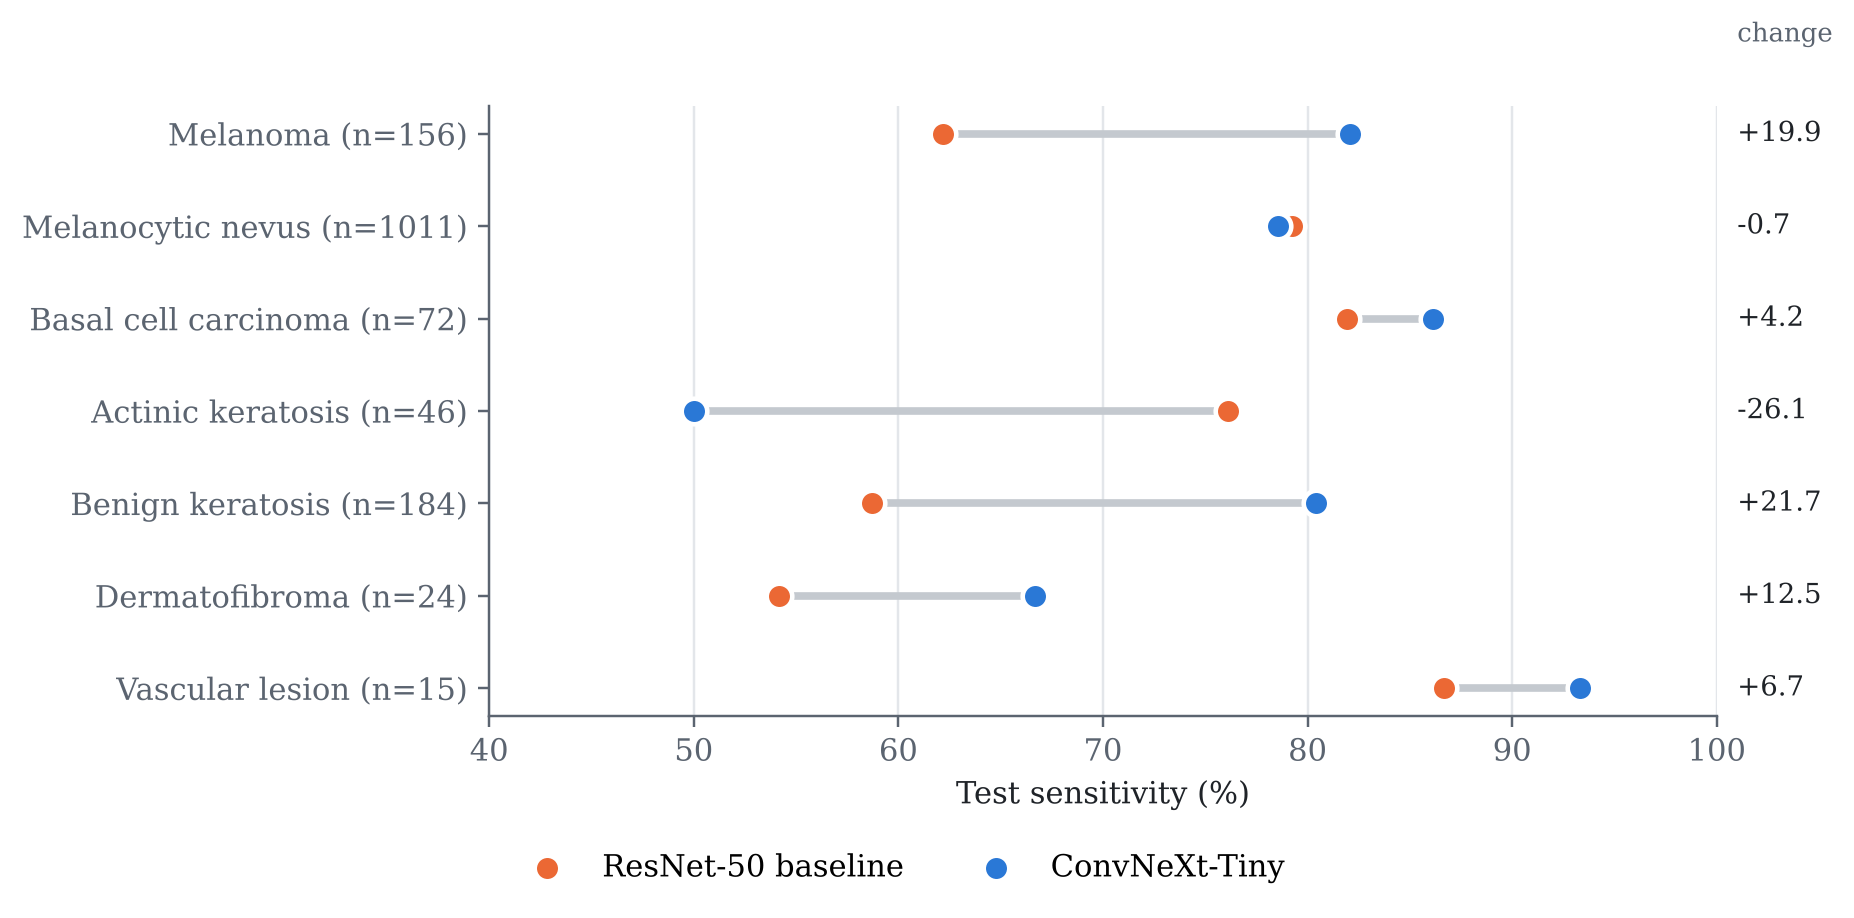
\includegraphics[width=0.82\textwidth]{fig_per_class.png}
\caption{Test-set sensitivity per class for both models, with the change in percentage points. Rare classes rest on few images (15 vascular lesions, 24 dermatofibromas), so their changes are uncertain.}
\label{fig:perclass}
\end{figure}

\begin{table}[ht]
\centering
\caption{Per-class test results of ConvNeXt-Tiny.}
\label{tab:perclass}
\small
\begin{tabular}{@{}lrrrrr@{}}
\toprule
Class & Test images & Specificity & F1 & ROC-AUC & Average precision \\
\midrule
Melanoma & 156 & 86.8\pct & 0.554 & 0.933 & 0.655 \\
Melanocytic nevus & 1,011 & 94.8\pct & 0.867 & 0.959 & 0.977 \\
Basal cell carcinoma & 72 & 98.3\pct & 0.780 & 0.988 & 0.825 \\
Actinic keratosis & 46 & 99.2\pct & 0.575 & 0.945 & 0.641 \\
Benign keratosis & 184 & 94.4\pct & 0.729 & 0.952 & 0.825 \\
Dermatofibroma & 24 & 99.6\pct & 0.696 & 0.984 & 0.779 \\
Vascular lesion & 15 & 99.8\pct & 0.875 & 0.999 & 0.954 \\
\bottomrule
\end{tabular}
\end{table}

\subsection{Melanoma screening operating point}
The threshold chosen on validation data transferred well to the test set (Table~\ref{tab:screen}). For ConvNeXt, a melanoma probability of 0.217 or more flagged 94.2\pct{} of test melanomas, slightly above the 90\pct{} target, while 75.5\pct{} of non-melanoma images were correctly left unflagged. At comparable sensitivity, the baseline's specificity was 11.9 points lower. In the malignant-versus-benign view, ConvNeXt reached 93.4\pct{} sensitivity at 73.9\pct{} specificity, with an AUC of 0.931 (baseline: 90.9\pct, 73.3\pct, 0.906).

\begin{table}[ht]
\centering
\caption{Melanoma screening at a threshold fixed on the validation set for at least 90\pct{} sensitivity.}
\label{tab:screen}
\small
\begin{tabular}{@{}lrcccc@{}}
\toprule
Model & Threshold & \makecell{Validation\\sens.\ / spec.} & \makecell{Test sensitivity\\(95\pct{} CI)} & \makecell{Test\\specificity} & \makecell{Melanoma\\ROC-AUC} \\
\midrule
ResNet-50 baseline & 0.067 & 90.5\pct{} / 59.5\pct & 91.0\pct{} (86.4--95.2) & 63.6\pct & 0.869 \\
ConvNeXt-Tiny & 0.217 & 90.5\pct{} / 71.2\pct & 94.2\pct{} (90.4--97.5) & 75.5\pct & 0.933 \\
\bottomrule
\end{tabular}
\end{table}

\subsection{Error analysis}
The most frequent error was a nevus predicted as melanoma: 150 of 1,011 nevi (14.8\pct; Figure~\ref{fig:confusion}). As a result, only 128 of the 306 images predicted as melanoma were melanomas (precision 41.8\pct). Of the 28 melanomas missed at the argmax rule, 17 were called nevi and 7 benign keratoses. Actinic keratoses were confused mainly with benign keratosis (11 images) and basal cell carcinoma (8). Fifty nevi were predicted as benign keratosis. A t-SNE projection of the model's embeddings shows the same overlap between melanoma, nevus and benign keratosis (Supplementary Figure~S3).

\begin{figure}[ht]
\centering
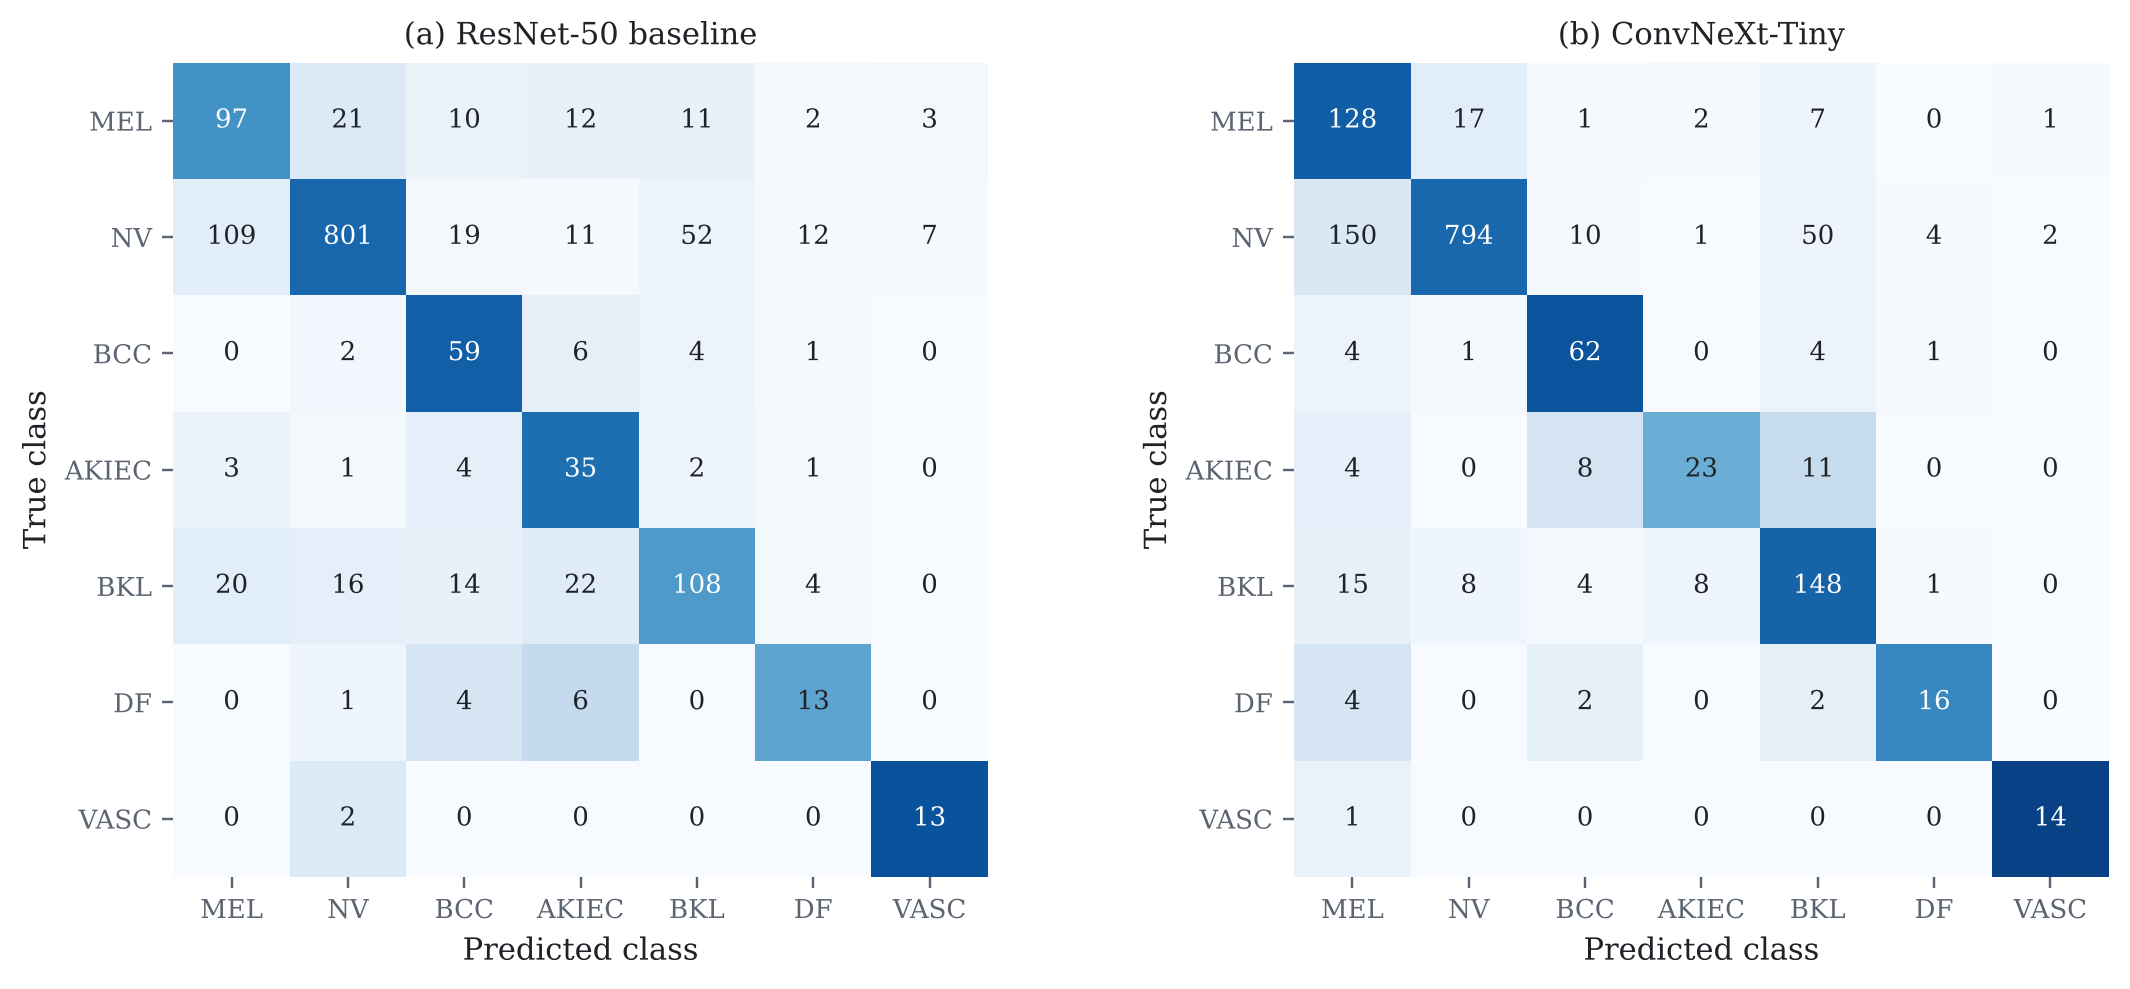
\includegraphics[width=\textwidth]{fig_confusion.png}
\caption{Confusion matrices on the test set for (a) the ResNet-50 baseline and (b) ConvNeXt-Tiny. Numbers are image counts; shading is the share of each true class.}
\label{fig:confusion}
\end{figure}

\subsection{Grad-CAM}
In 13 of the 14 inspected test images, the Grad-CAM maps lay on the lesion rather than on rulers, hair or the dark corners of the dermatoscope (Figure~\ref{fig:gradcam}); one dermatofibroma map also showed a small hot spot at the image edge. For melanomas with several dark regions, the maps covered several separate areas at the lesion periphery. Three of the 14 images were misclassified: a benign keratosis called melanoma, a benign keratosis called a nevus, and an actinic keratosis called a benign keratosis. In these, the maps were as focused as in correct cases, so map appearance alone did not reveal the error.

\begin{figure}[ht]
\centering
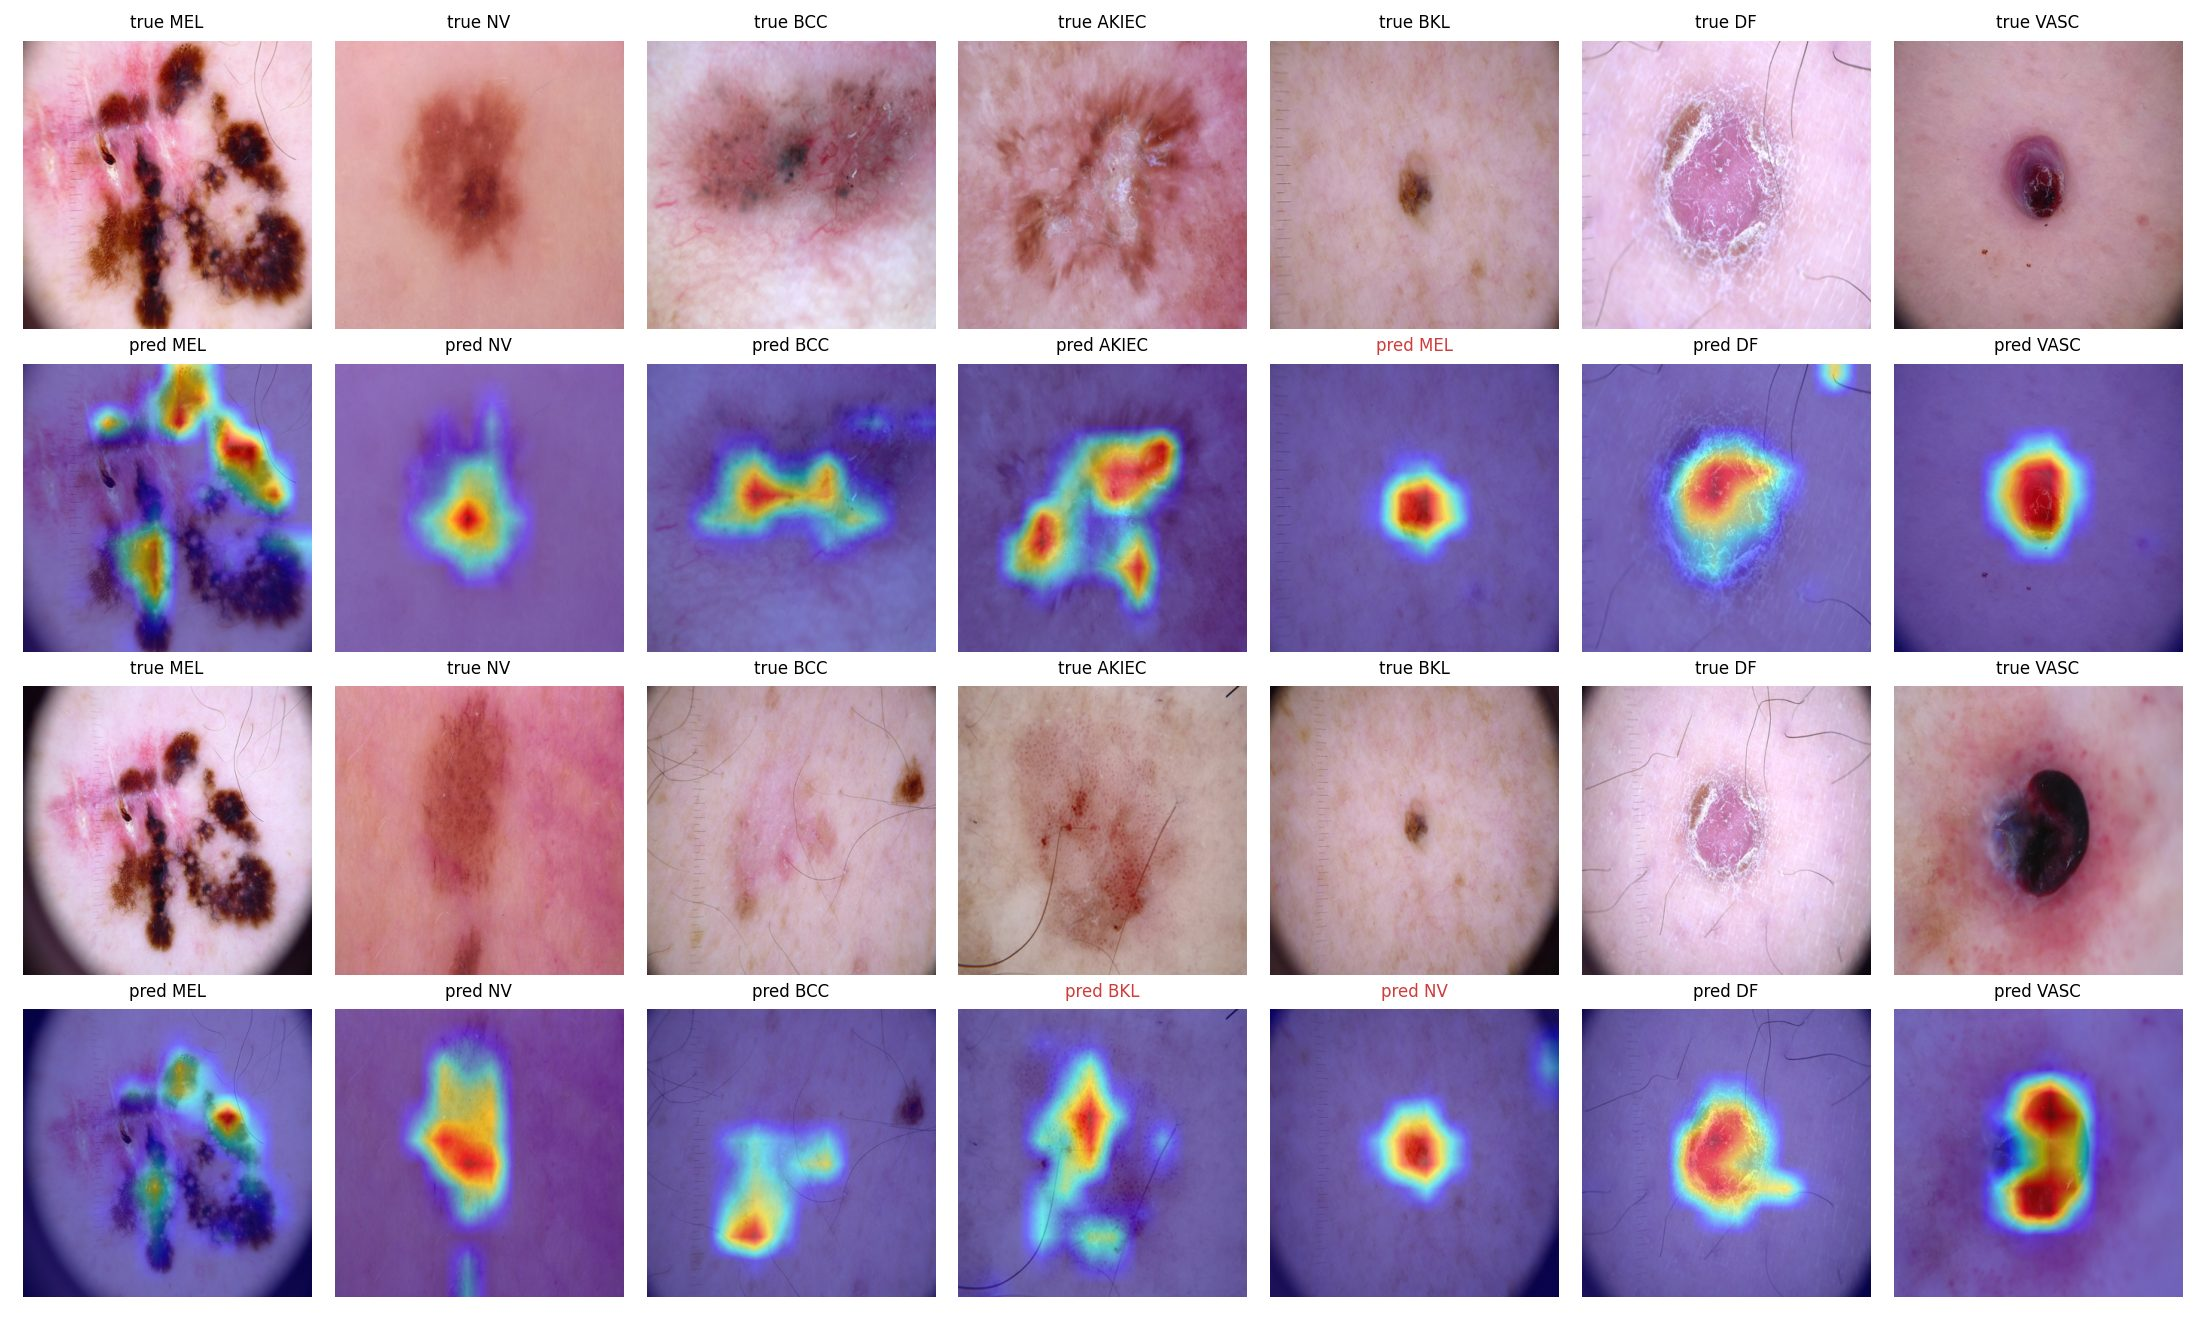
\includegraphics[width=\textwidth]{fig_gradcam.jpg}
\caption{Test images (rows 1 and 3) and Grad-CAM maps for the predicted class of ConvNeXt-Tiny (rows 2 and 4), two images per class. Titles give the true and predicted class; red titles mark errors.}
\label{fig:gradcam}
\end{figure}

% ------------------------------------------------------------------ 5
\section{Discussion}
\subsection{Principal findings}
Under a lesion-grouped protocol with a test set used once, ConvNeXt-Tiny with class-balanced sampling detected 82.1\pct{} of melanomas as its top prediction, against 62.2\pct{} for a capstone-style ResNet-50. A threshold fixed on validation data for 90\pct{} sensitivity gave 94.2\pct{} sensitivity on the test set, so the operating point transferred rather than having been tuned to the test images. Macro-AUC improved from 0.932 to 0.966 with non-overlapping intervals.

\subsection{What the comparison can and cannot show}
The two models differ in architecture, input resolution, imbalance handling, augmentation, label smoothing and test-time augmentation. I did not run ablations, so the improvement cannot be attributed to any single change. Higher resolution and balanced sampling are plausible main contributors, since melanoma and benign keratosis gained most, but this remains a hypothesis.

The baseline in this study detected 62.2\pct{} of melanomas, while the original capstone model reported 36.3\pct{} on an image-level split. Leakage would be expected to inflate the capstone figure, not lower it. The gap therefore most likely reflects training differences, such as the capstone's partly frozen backbone, rather than the split. It also shows that a figure from a single, unaudited pipeline says little about what a design can achieve.

My numbers are not directly comparable with the ISIC 2018 leaderboard, which was scored on the official test set and often used ensembles and external data. My test set is internal, drawn from the same clinics as the training data, and therefore likely easier than truly new data \cite{tschandl2019}.

\subsection{Errors that matter for triage}
The main cost of higher melanoma sensitivity was false alarms on nevi: 14.8\pct{} of nevi were predicted as melanoma. At the screening threshold, 331 of the 1,352 non-melanoma test images were flagged together with 147 melanomas. With the test set's 10.3\pct{} melanoma prevalence, about 31\pct{} of flagged images were melanomas. In primary care, where melanoma prevalence among examined lesions is far lower, this proportion would fall further, so flagged cases need specialist review rather than direct biopsy.

Actinic keratosis sensitivity fell by 26.1 points, with errors spread to benign keratosis and basal cell carcinoma, both keratinocytic lesions with overlapping dermoscopic features. Possible causes include overfitting to the 221 oversampled training images and the noisy, early model selection seen in the validation curve. Because actinic keratosis can progress to squamous cell carcinoma, this weakness matters clinically. Class-specific thresholds, several training seeds and clinical metadata such as age and body site are direct next steps.

\subsection{Explainability and the prototype}
Grad-CAM maps were mostly centred on the lesion, which argues against reliance on obvious artefacts such as rulers or vignetting. Maps of misclassified images looked as plausible as those of correct ones, so Grad-CAM supports inspection but cannot flag errors on its own. The ABCD descriptors and similar-case retrieval in the prototype are aids for discussion between a health assistant and a dermatologist. They were not validated and should not drive decisions.

\subsection{Limitations}
\begin{itemize}
  \item All images come from one public dataset, mostly from clinics in Austria and Australia and from patients with lighter skin. Models of this kind lose substantial performance on darker skin tones \cite{daneshjou2022}, and performance on patients in Nepal is unknown.
  \item The test set is an internal held-out split, not an external or prospective cohort, and the official ISIC 2018 test labels were not used.
  \item Each model was trained once with one seed, and hyperparameters were not tuned.
  \item Bootstrap intervals resample images rather than lesions; with 1,508 images from 1,120 lesions, they may be slightly too narrow.
  \item The dermatofibroma and vascular classes have 24 and 15 test images, and the validation set holds only 10 dermatofibromas.
  \item The prototype application has not been evaluated with clinicians or patients.
\end{itemize}

\subsection{Future work}
The priorities are an external validation on dermoscopic images collected in Nepali hospitals, including darker skin types, and ablations that separate the effects of architecture, resolution and sampling. Further steps include probability calibration, several seeds, evaluation on the official ISIC 2018 test set, and a usability study of the triage application with health assistants.

% ------------------------------------------------------------------ 6
\section{Conclusion}
Evaluated on lesions it had never seen, a ConvNeXt-Tiny classifier with class-balanced sampling reached 76.7\pct{} balanced accuracy on seven-class dermoscopic diagnosis and flagged 94.2\pct{} of melanomas at 75.5\pct{} specificity with a threshold fixed in advance. Grouping by lesion, selecting on validation data only and reporting confidence intervals are simple steps, and they change what a HAM10000 result can be trusted to mean. The remaining weaknesses, in actinic keratosis, nevus false alarms and unknown performance on South Asian skin, define the next study: external validation in Nepali clinics before any clinical use. Code, the split, results and the trained model are openly available.

% ------------------------------------------------------------------ declarations
\section*{Declarations}
\small\sloppy
\textbf{Data availability.} HAM10000 is publicly available from the Harvard Dataverse (doi:10.7910/DVN/DBW86T) under a CC BY-NC 4.0 licence. The lesion-grouped split, all test metrics and the trained ConvNeXt-Tiny weights are available in the code repository.

\textbf{Code availability.} \url{https://github.com/subarna007/skin-lesion-classification-isic2018}

\textbf{Ethics approval and consent.} This study used only a public, de-identified dataset. No new human data were collected, so ethics approval and informed consent were not required. The hospital in the prototype is fictional and the application was not used with patients.

\textbf{Funding.} This research received no external funding.

\textbf{Competing interests.} The author declares no competing interests.

\textbf{Reporting.} The manuscript was prepared with reference to the Checklist for Artificial Intelligence in Medical Imaging (CLAIM) \cite{mongan2020}; Supplementary Table~S2 shows where its main items are addressed.

\normalsize
% ------------------------------------------------------------------ references
\renewcommand{\refname}{References}
\begin{thebibliography}{99}
\small
\setlength{\itemsep}{0.15em}
\bibitem{bray2024} Bray F, Laversanne M, Sung H, Ferlay J, Siegel RL, Soerjomataram I, Jemal A. Global cancer statistics 2022: GLOBOCAN estimates of incidence and mortality worldwide for 36 cancers in 185 countries. \emph{CA Cancer J Clin}. 2024;74(3):229--263. doi:10.3322/caac.21834
\bibitem{iarc2024} International Agency for Research on Cancer. Melanoma of skin fact sheet. Global Cancer Observatory, GLOBOCAN 2022; 2024. \url{https://gco.iarc.who.int}
\bibitem{freeman2026} Freeman EE, Yardman-Frank JM, Kilmer J, et al. Global disparities in access to dermatological care. \emph{JAMA Dermatol}. Published online August 26, 2026. doi:10.1001/jamadermatol.2026.3112
\bibitem{esteva2017} Esteva A, Kuprel B, Novoa RA, Ko J, Swetter SM, Blau HM, Thrun S. Dermatologist-level classification of skin cancer with deep neural networks. \emph{Nature}. 2017;542(7639):115--118. doi:10.1038/nature21056
\bibitem{haenssle2018} Haenssle HA, Fink C, Schneiderbauer R, et al. Man against machine: diagnostic performance of a deep learning convolutional neural network for dermoscopic melanoma recognition in comparison to 58 dermatologists. \emph{Ann Oncol}. 2018;29(8):1836--1842. doi:10.1093/annonc/mdy166
\bibitem{tschandl2019} Tschandl P, Codella N, Akay BN, et al. Comparison of the accuracy of human readers versus machine-learning algorithms for pigmented skin lesion classification: an open, web-based, international, diagnostic study. \emph{Lancet Oncol}. 2019;20(7):938--947. doi:10.1016/S1470-2045(19)30333-X
\bibitem{codella2019} Codella N, Rotemberg V, Tschandl P, et al. Skin lesion analysis toward melanoma detection 2018: a challenge hosted by the International Skin Imaging Collaboration (ISIC). arXiv:1902.03368; 2019.
\bibitem{tschandl2018} Tschandl P, Rosendahl C, Kittler H. The HAM10000 dataset, a large collection of multi-source dermatoscopic images of common pigmented skin lesions. \emph{Sci Data}. 2018;5:180161. doi:10.1038/sdata.2018.161
\bibitem{cassidy2022} Cassidy B, Kendrick C, Brodzicki A, Jaworek-Korjakowska J, Yap MH. Analysis of the ISIC image datasets: usage, benchmarks and recommendations. \emph{Med Image Anal}. 2022;75:102305. doi:10.1016/j.media.2021.102305
\bibitem{abhishek2025} Abhishek K, Jain A, Hamarneh G. Investigating the quality of DermaMNIST and Fitzpatrick17k dermatological image datasets. \emph{Sci Data}. 2025;12:196. doi:10.1038/s41597-025-04382-5
\bibitem{daneshjou2022} Daneshjou R, Vodrahalli K, Novoa RA, et al. Disparities in dermatology AI performance on a diverse, curated clinical image set. \emph{Sci Adv}. 2022;8(32):eabq6147. doi:10.1126/sciadv.abq6147
\bibitem{he2016} He K, Zhang X, Ren S, Sun J. Deep residual learning for image recognition. In: \emph{Proc IEEE Conf Computer Vision and Pattern Recognition (CVPR)}; 2016:770--778.
\bibitem{liu2022} Liu Z, Mao H, Wu CY, Feichtenhofer C, Darrell T, Xie S. A ConvNet for the 2020s. In: \emph{Proc IEEE/CVF Conf Computer Vision and Pattern Recognition (CVPR)}; 2022:11976--11986.
\bibitem{selvaraju2017} Selvaraju RR, Cogswell M, Das A, Vedantam R, Parikh D, Batra D. Grad-CAM: visual explanations from deep networks via gradient-based localization. In: \emph{Proc IEEE Int Conf Computer Vision (ICCV)}; 2017:618--626.
\bibitem{loshchilov2019} Loshchilov I, Hutter F. Decoupled weight decay regularization. In: \emph{Int Conf Learning Representations (ICLR)}; 2019.
\bibitem{szegedy2016} Szegedy C, Vanhoucke V, Ioffe S, Shlens J, Wojna Z. Rethinking the Inception architecture for computer vision. In: \emph{Proc IEEE Conf Computer Vision and Pattern Recognition (CVPR)}; 2016:2818--2826.
\bibitem{efron1993} Efron B, Tibshirani RJ. \emph{An Introduction to the Bootstrap}. New York: Chapman \& Hall; 1993.
\bibitem{nachbar1994} Nachbar F, Stolz W, Merkle T, et al. The ABCD rule of dermatoscopy: high prospective value in the diagnosis of doubtful melanocytic skin lesions. \emph{J Am Acad Dermatol}. 1994;30(4):551--559.
\bibitem{abbasi2004} Abbasi NR, Shaw HM, Rigel DS, et al. Early diagnosis of cutaneous melanoma: revisiting the ABCD criteria. \emph{JAMA}. 2004;292(22):2771--2776.
\bibitem{wightman2019} Wightman R. PyTorch Image Models. GitHub repository; 2019. doi:10.5281/zenodo.4414861
\bibitem{otsu1979} Otsu N. A threshold selection method from gray-level histograms. \emph{IEEE Trans Syst Man Cybern}. 1979;9(1):62--66.
\bibitem{pedregosa2011} Pedregosa F, Varoquaux G, Gramfort A, et al. Scikit-learn: machine learning in Python. \emph{J Mach Learn Res}. 2011;12:2825--2830.
\bibitem{paszke2019} Paszke A, Gross S, Massa F, et al. PyTorch: an imperative style, high-performance deep learning library. In: \emph{Advances in Neural Information Processing Systems 32 (NeurIPS)}; 2019:8024--8035.
\bibitem{vandermaaten2008} van der Maaten L, Hinton G. Visualizing data using t-SNE. \emph{J Mach Learn Res}. 2008;9:2579--2605.
\bibitem{mongan2020} Mongan J, Moy L, Kahn CE Jr. Checklist for Artificial Intelligence in Medical Imaging (CLAIM): a guide for authors and reviewers. \emph{Radiol Artif Intell}. 2020;2(2):e200029. doi:10.1148/ryai.2020200029
\end{thebibliography}

% ------------------------------------------------------------------ supplementary
\clearpage
\setcounter{figure}{0}
\setcounter{table}{0}
\renewcommand{\thefigure}{S\arabic{figure}}
\renewcommand{\thetable}{S\arabic{table}}
\fancyhead[R]{\small\itshape Supplementary material}

\begin{center}
{\Large\bfseries Supplementary material\par}
\end{center}
This supplement gives the additional results, configuration and reproduction details needed to check the analysis. All numbers are read from the result files in the code repository (\texttt{results/*.json}).

\section*{Example images}
\begin{figure}[H]
\centering
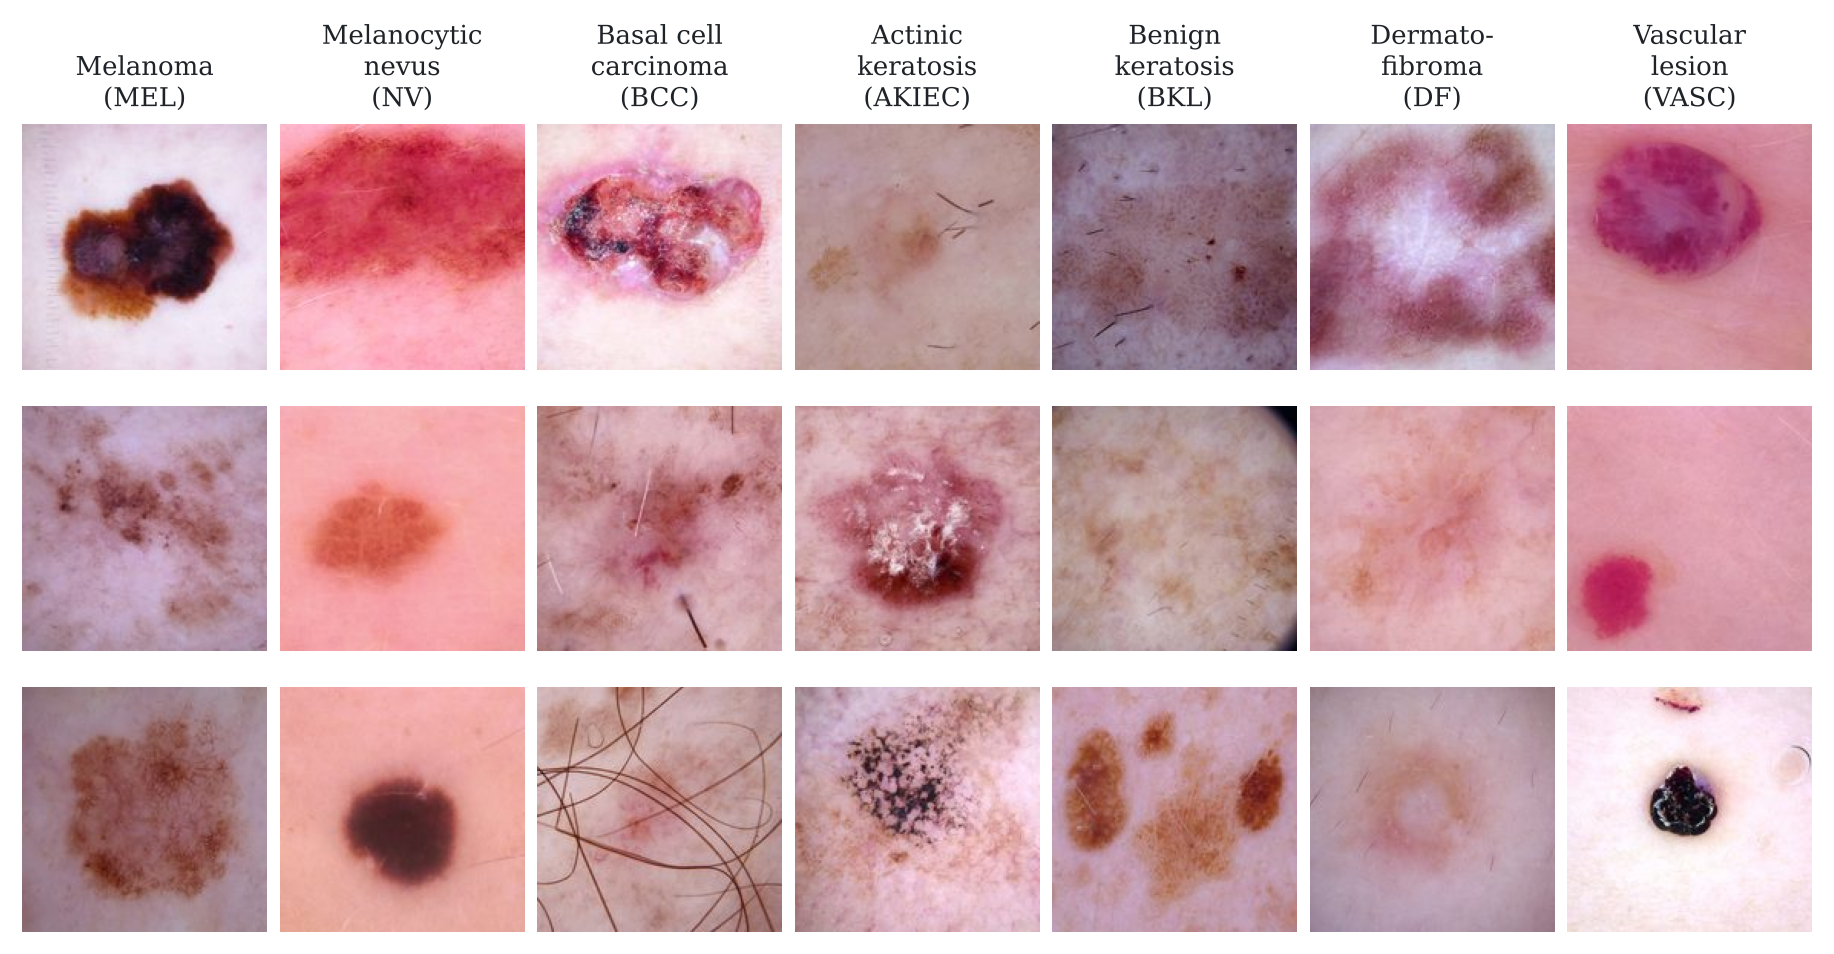
\includegraphics[width=\textwidth]{fig_samples.png}
\caption{Three example images per class from the HAM10000 training set \cite{tschandl2018}.}
\end{figure}

\section*{Full per-class results of both models}
\begin{table}[H]
\centering
\caption{Per-class test results of both models. Sens.\ = sensitivity, Spec.\ = specificity, Prec.\ = precision, AP = average precision.}
\small
\begin{tabular}{@{}llrrrrrrr@{}}
\toprule
Class & Model & Images & Sens. & Spec. & Prec. & F1 & AUC & AP \\
\midrule
\multirow{2}{*}{MEL} & ResNet-50 & 156 & 62.2\pct & 90.2\pct & 42.4\pct & 0.504 & 0.869 & 0.519 \\
 & ConvNeXt-Tiny & 156 & 82.1\pct & 86.8\pct & 41.8\pct & 0.554 & 0.933 & 0.655 \\
\midrule
\multirow{2}{*}{NV} & ResNet-50 & 1,011 & 79.2\pct & 91.3\pct & 94.9\pct & 0.864 & 0.945 & 0.971 \\
 & ConvNeXt-Tiny & 1,011 & 78.5\pct & 94.8\pct & 96.8\pct & 0.867 & 0.959 & 0.977 \\
\midrule
\multirow{2}{*}{BCC} & ResNet-50 & 72 & 81.9\pct & 96.4\pct & 53.6\pct & 0.648 & 0.968 & 0.689 \\
 & ConvNeXt-Tiny & 72 & 86.1\pct & 98.3\pct & 71.3\pct & 0.780 & 0.988 & 0.825 \\
\midrule
\multirow{2}{*}{AKIEC} & ResNet-50 & 46 & 76.1\pct & 96.1\pct & 38.0\pct & 0.507 & 0.953 & 0.559 \\
 & ConvNeXt-Tiny & 46 & 50.0\pct & 99.2\pct & 67.6\pct & 0.575 & 0.945 & 0.641 \\
\midrule
\multirow{2}{*}{BKL} & ResNet-50 & 184 & 58.7\pct & 94.8\pct & 61.0\pct & 0.598 & 0.869 & 0.602 \\
 & ConvNeXt-Tiny & 184 & 80.4\pct & 94.4\pct & 66.7\pct & 0.729 & 0.952 & 0.825 \\
\midrule
\multirow{2}{*}{DF} & ResNet-50 & 24 & 54.2\pct & 98.7\pct & 39.4\pct & 0.456 & 0.926 & 0.554 \\
 & ConvNeXt-Tiny & 24 & 66.7\pct & 99.6\pct & 72.7\pct & 0.696 & 0.984 & 0.779 \\
\midrule
\multirow{2}{*}{VASC} & ResNet-50 & 15 & 86.7\pct & 99.3\pct & 56.5\pct & 0.684 & 0.992 & 0.893 \\
 & ConvNeXt-Tiny & 15 & 93.3\pct & 99.8\pct & 82.4\pct & 0.875 & 0.999 & 0.954 \\
\bottomrule
\end{tabular}
\end{table}

\section*{Training curves}
\begin{figure}[H]
\centering
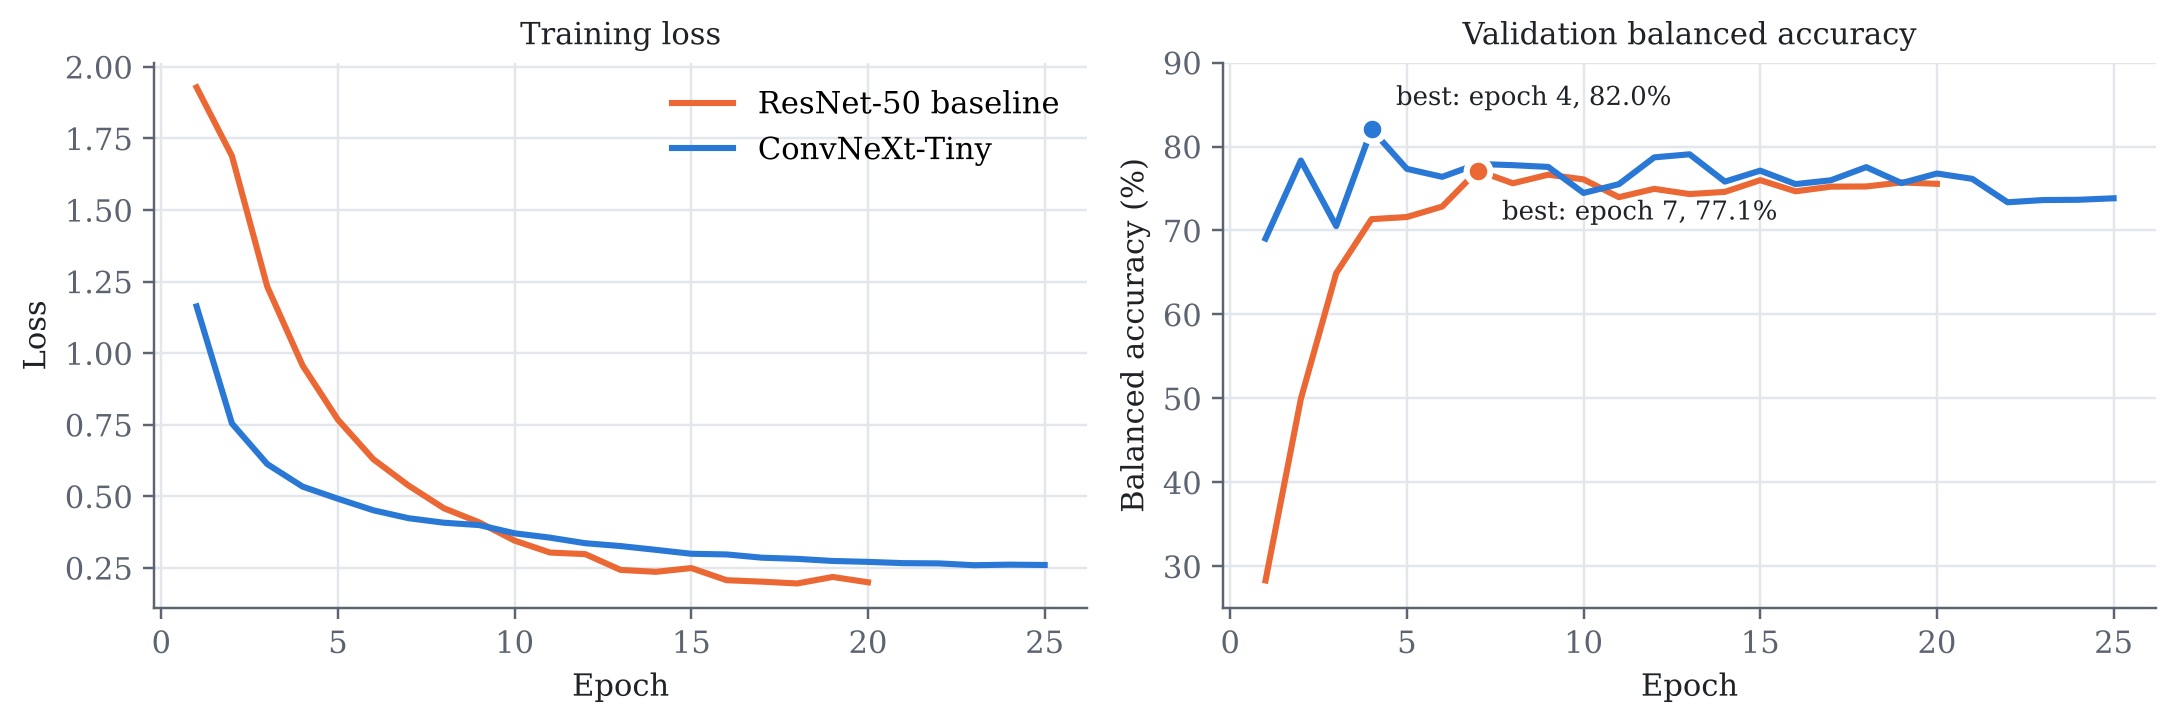
\includegraphics[width=\textwidth]{fig_training_curves.png}
\caption{Training loss and validation balanced accuracy per epoch. Dots mark the epoch kept for testing. The loss curves are not directly comparable, because the baseline uses a class-weighted loss and ConvNeXt a label-smoothed loss with balanced sampling.}
\end{figure}

\section*{Feature-space projection}
\begin{figure}[H]
\centering
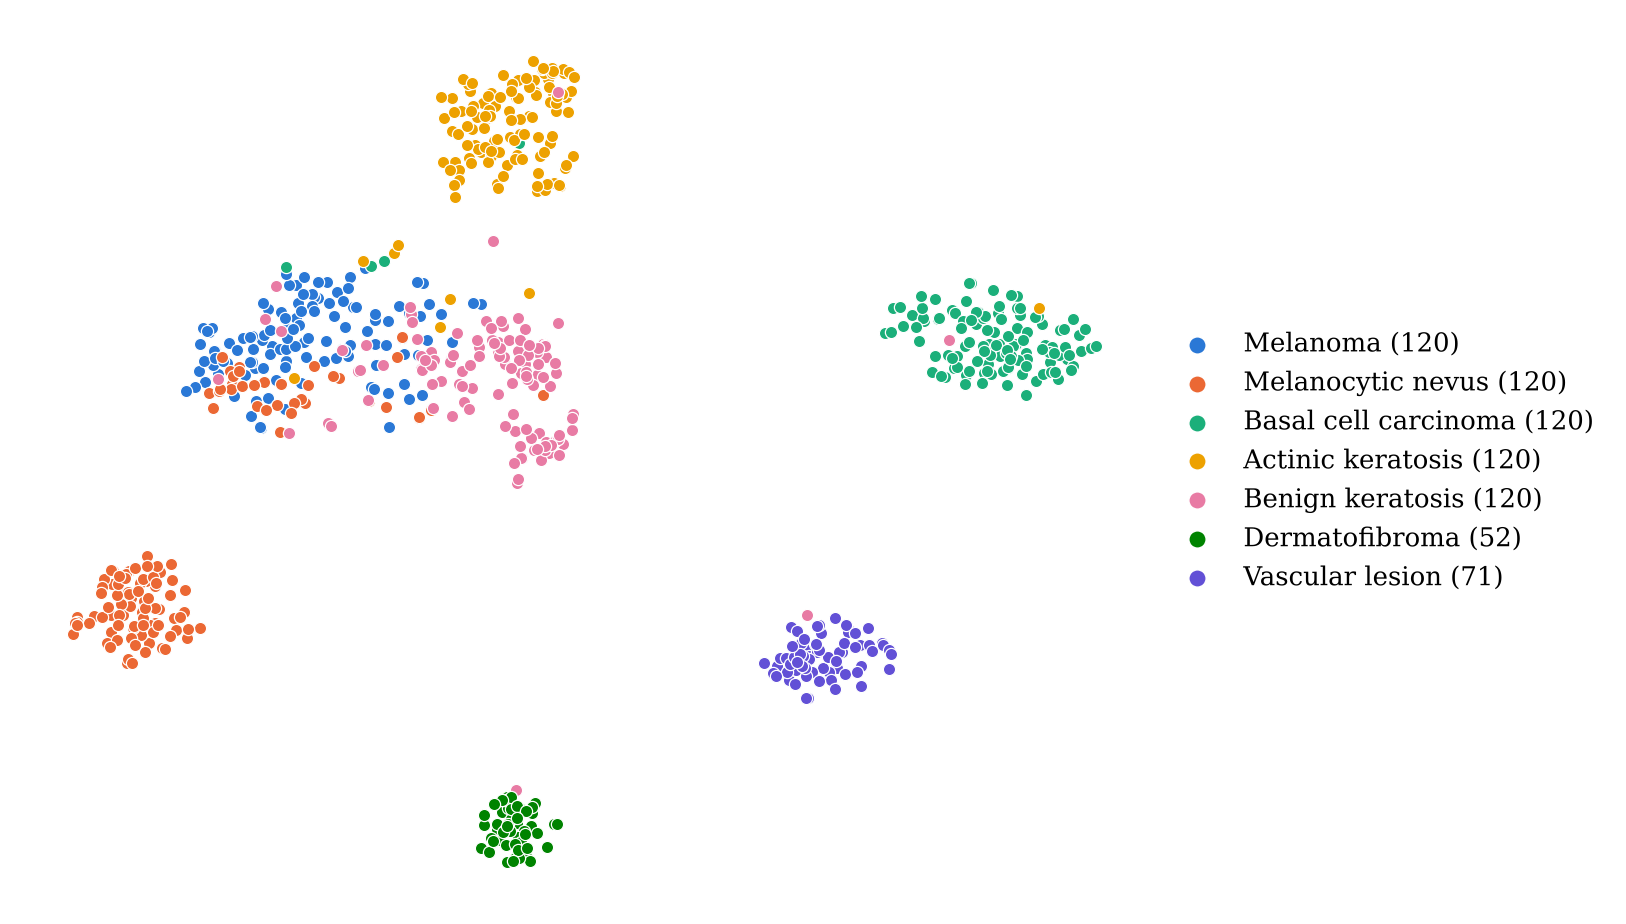
\includegraphics[width=0.8\textwidth]{fig_tsne.png}
\caption{t-SNE projection \cite{vandermaaten2008} of ConvNeXt-Tiny pre-logit embeddings for the 723 gallery images (training images, one per lesion). Vascular lesions, dermatofibromas, basal cell carcinomas and actinic keratoses form separate clusters, while melanomas, nevi and benign keratoses overlap, matching the main test errors. Because the model was trained on these images, the separation overstates what it achieves on new images.}
\end{figure}

\section*{Prototype application}
\begin{figure}[H]
\centering
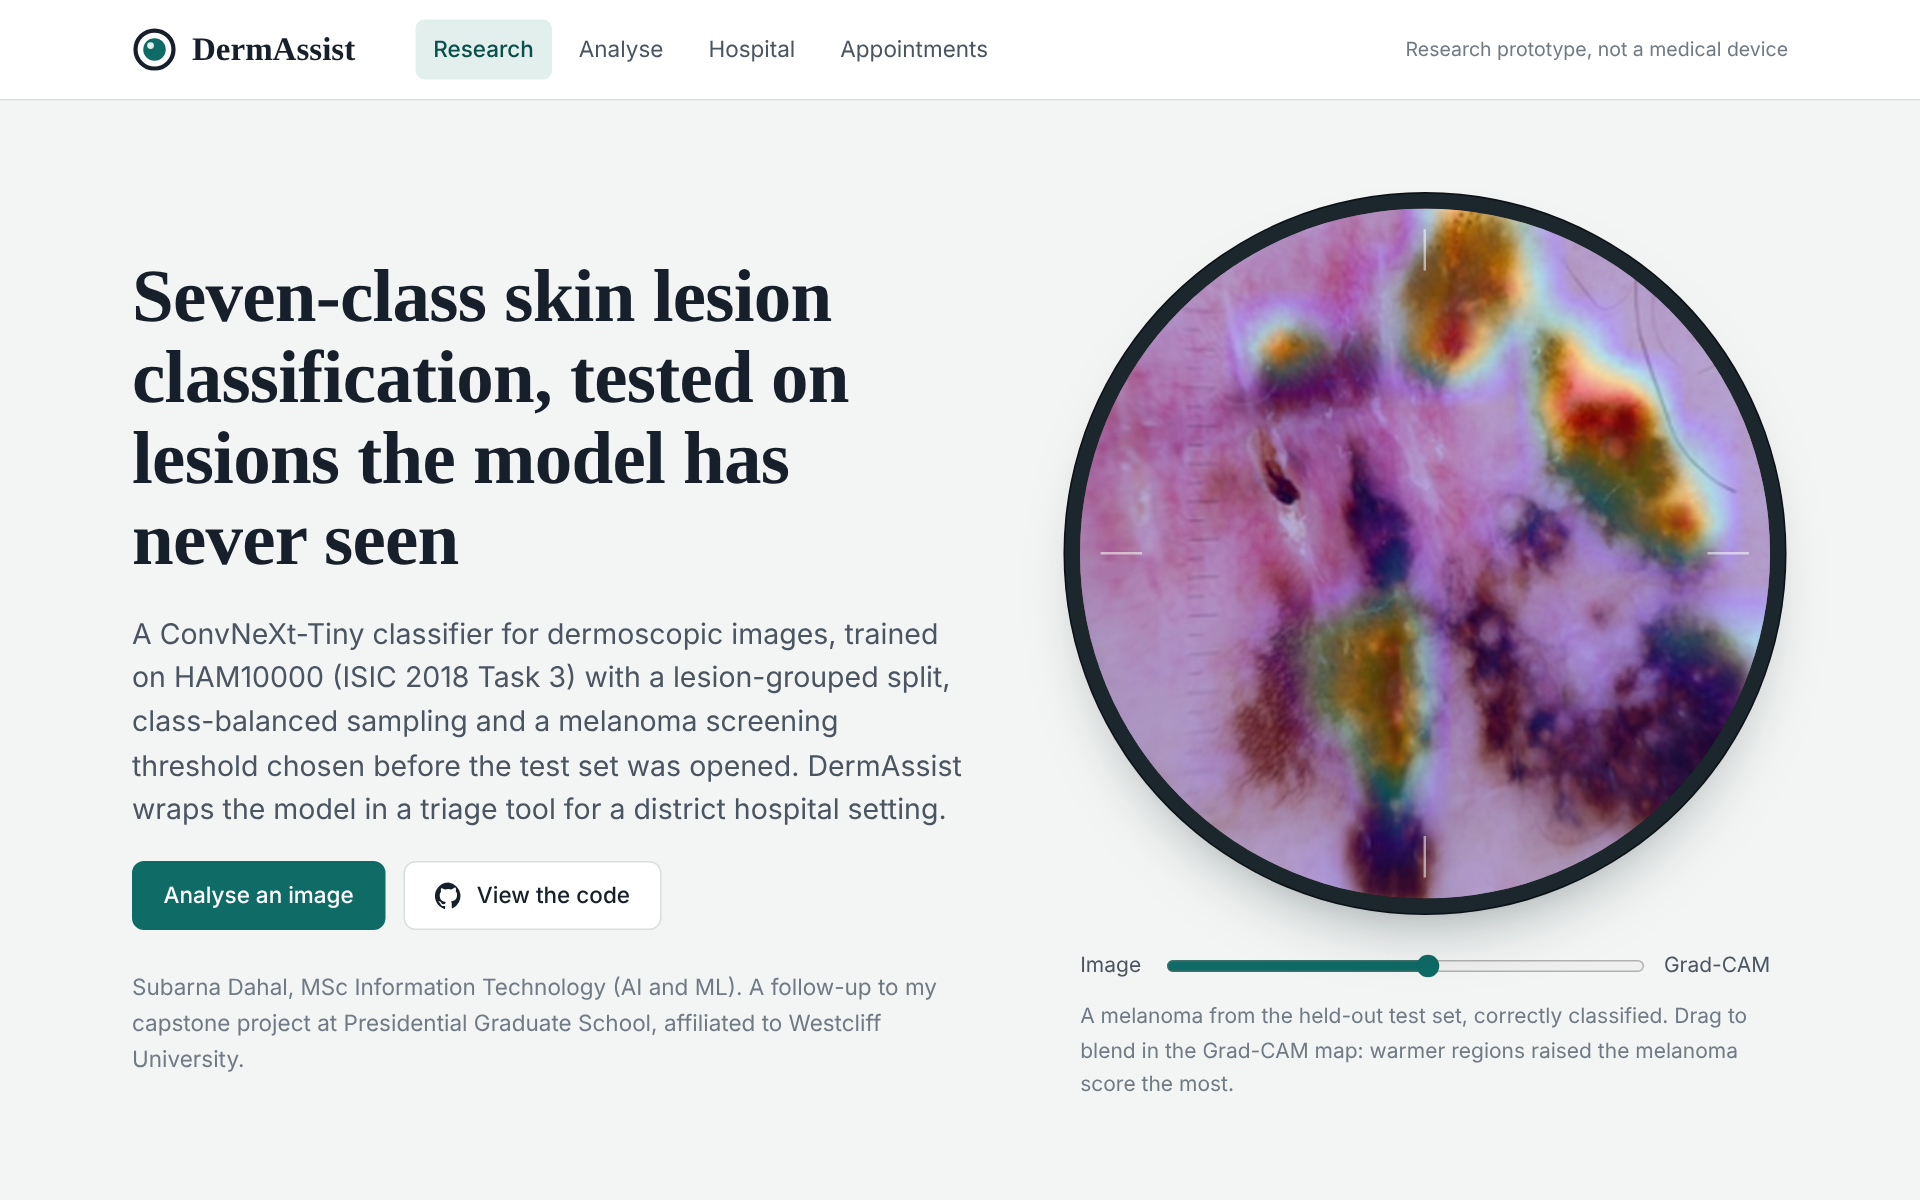
\includegraphics[width=0.85\textwidth]{web_home.png}
\caption{The start page of the DermAssist prototype. A slider blends the Grad-CAM map over a correctly classified test melanoma. The application also has pages to analyse an image, a review queue for a fictional district hospital and an appointment booking page.}
\end{figure}

\section*{Similar-case retrieval}
\begin{figure}[H]
\centering
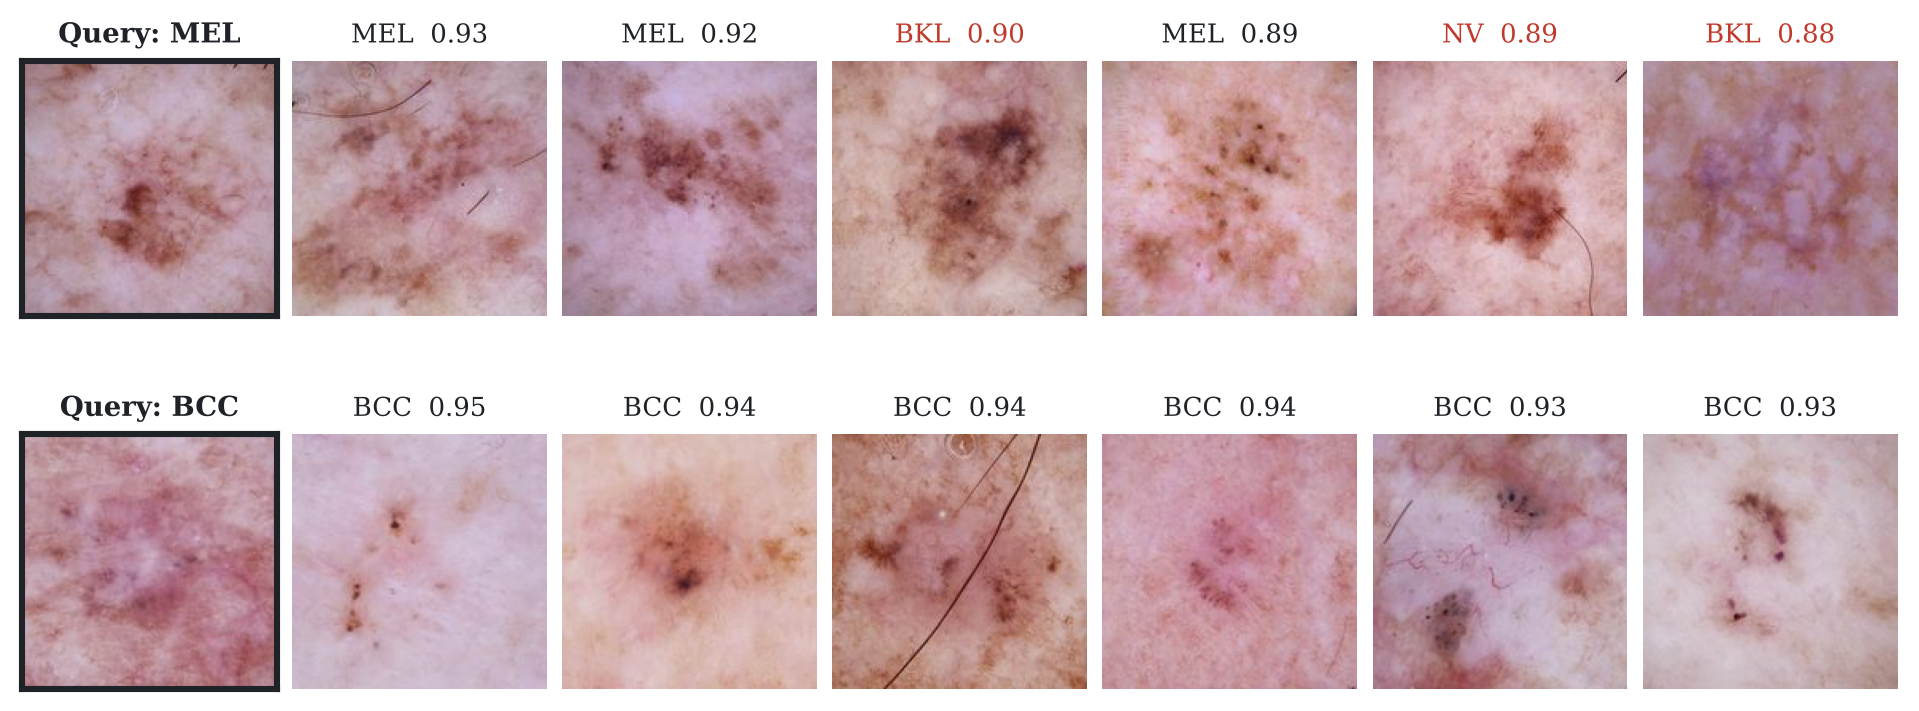
\includegraphics[width=\textwidth]{fig_similar.png}
\caption{Six nearest gallery images by cosine similarity of the ConvNeXt-Tiny embeddings, for a melanoma (top) and a basal cell carcinoma (bottom) query. Red titles mark a different diagnosis from the query.}
\end{figure}

\section*{Reproducibility}
\sloppy
\textbf{Configurations.} Each run stores its full configuration with its results:
\begin{itemize}
  \item \texttt{baseline\_resnet50}: arch resnet50, image size 224, 20 epochs, batch 32, learning rate $10^{-4}$, weight decay $10^{-4}$, weighted cross-entropy, no label smoothing, no sampler, basic augmentation, no TTA, seed 42.
  \item \texttt{convnext\_balanced}: arch convnext\_tiny, image size 384, 25 epochs, batch 32, learning rate $10^{-4}$, weight decay 0.05, cross-entropy with label smoothing 0.05, balanced sampler, strong augmentation, flip TTA, seed 42.
\end{itemize}
\textbf{Running the experiments.} \texttt{pip install -r requirements.txt} then \texttt{bash run\_all.sh} builds the split, trains both models, evaluates them and writes all results to \texttt{results/}. On one T4 GPU, training takes 14.7 and 48.1 minutes. The prototype runs with \texttt{uvicorn app.server:app --port 8000}.

\textbf{Files in the repository.} \texttt{results/splits.csv} (split assignment of every image), \texttt{results/*.json} (all metrics, confidence intervals, confusion matrices and operating points), \texttt{checkpoints/} (trained ConvNeXt-Tiny weights), \texttt{src/} (code for every step).

\section*{Reporting checklist summary}
\begin{table}[H]
\centering
\caption{Where the main items of the CLAIM checklist \cite{mongan2020} are addressed.}
\small
\begin{tabularx}{\textwidth}{@{}lX@{}}
\toprule
Item & Where addressed \\
\midrule
Study design and intended use & Sections 1 and 3.7; screening and triage support, not diagnosis \\
Data source, inclusion and labels & Section 3.1; HAM10000, all 10,015 images, histopathology or follow-up labels \\
Data partitions and leakage prevention & Section 3.2, Figure 1, Table 1; split grouped by lesion \\
Preprocessing and augmentation & Section 3.3, Table 2 \\
Model architecture and initialisation & Section 3.3; ImageNet-pretrained ResNet-50 and ConvNeXt-Tiny \\
Training details and hyperparameters & Section 3.3, Table 2, Supplement (Reproducibility) \\
Model selection & Section 3.4; validation balanced accuracy only \\
Operating point & Section 3.4, Table 5; threshold fixed on validation data \\
Metrics and statistical uncertainty & Section 3.5; bootstrap 95\pct{} confidence intervals \\
Per-class performance and failure analysis & Sections 4.2 and 4.4, Figures 2--3, Table S1 \\
Explainability & Sections 3.6 and 4.5, Figure 4 \\
External validation & Not performed; stated in Section 5.5 \\
Limitations and generalisability & Section 5.5 \\
Code, data and model availability & Declarations; public repository \\
\bottomrule
\end{tabularx}
\end{table}

\end{document}
